% $Author: stef $
% $Date: 2008-04-04 17:14:31 +0200 (Fri, 04 Apr 2008) $
% $Revision: 318 $
%=================================================================
\ifx\wholebook\relax\else
% --------------------------------------------
% Lulu:
    \documentclass[a4paper,10pt,twoside]{book}
    \usepackage[
        papersize={6in,9in},
        hmargin={.75in,.75in},
        vmargin={.75in,1in},
        ignoreheadfoot
    ]{geometry}
    \input{../common.tex}
    \pagestyle{headings}
    \setboolean{lulu}{true}
% --------------------------------------------
% A4:
%   \documentclass[a4paper,11pt,twoside]{book}
%   \input{../common.tex}
%   \usepackage{a4wide}
% --------------------------------------------
    \graphicspath{{figures/} {../figures/}}
    \begin{document}
%   \renewcommand{\nnbb}[2]{} % Disable editorial comments
    \sloppy
\fi

\chapter{Methods: Named Message Sequences}\label{cha:methods}

Up to now, you have been using scripts to create robots and send them sequences of messages. 
Using scripts has the advantage of being a straightforward approach, but it has some 
severe limitations. One of the major limitations is that a script cannot be called by another 
script. This is a serious problem, because a script cannot be reused by other scripts. You have 
to rewrite the same sequence of messages again and again. 

Wouldn’t it be nice if one could define a kind of script whose sequence of messages could 
be sent to any robot? In fact, this is possible, and such a sequence of messages is called a 
\emph{method}. (In the context of this book we will not go into the full power of methods, since that 
would get us into the somewhat tricky subject of object-oriented programming.) A \emph{method} is 
a named script. The name of a method can be used in a script or even in another method to 
invoke the method. Actually, there is nothing much new here: all the robot messages that you 
have used so far represent methods that you could use with any robot! 

In this chapter, you will learn how to define methods. You already know most of what you 
need to write the code of a method. However, a method must be defined using a special editor 
called a \emph{code browser}. We will start by comparing a script and a method. Then we will define a 
method, and finally, we will look in detail at what we have accomplished. 

\section{Scripts versus Methods}

Let’s look at one of the scripts that you have already written, for example, Script~\ref{scr:121}, which 
creates a robot and tells it to draw a square with side length 100 pixels. 

\begin{script}[121]{Pica draws a simple square.}
| pica | 
pica := Bot new. 
4 timesRepeat: 
	[ pica turnLeft: 90. 
	pica go: 100 ] 
\end{script}


The problem with this script is that each time you need to draw a square of side length 
100 you need to \emph{copy} the three last lines of Script~\ref{scr:121}. Furthermore, if you want another robot 
(for example, \emph{daly}) to draw the square, you must change the name \emph{pica} to \emph{daly} everywhere. 
This is illustrated by Script~\ref{scr:122}. 

\begin{script}[122]{Pica and daly each draw a simple square.}
| pica daly | 
pica := Bot new. 
daly := Bot new. 
daly jump: 200. 
daly color: Color red. 
!\textbf{4 timesRepeat:}!
	!\textbf{[ pica turnLeft: 90.}!
	!\textbf{pica go: 100 ].}!
!\textbf{4 timesRepeat:} !
	!\textbf{[ daly turnLeft: 90.} !
	!\textbf{daly go: 100 ].}!
\end{script}

For all these reasons, working with scripts is not easy. In fact, I suspect that the following 
three statements reflect your personal experience with scripts: 

\begin{itemize}
\item Writing long scripts is a painful task. 
\item Repeating long scripts is boring and error-prone. 
\item When one is copying complex scripts, the likelihood of making a programming error, such as omitting a line, is high. (A programming error is an error in the logic of a program. In contrast to syntax errors, which are caught quickly by the computer because they are errors in program structure, programming errors can be quite difficult to catch.)
\end{itemize}

To overcome these difficulties, we would like to \emph{define} a sequence of messages once and 
for all, give the sequence a \emph{name}, and then be able to send the \emph{named sequence} as a single 
message to any robot, just as we have been able to send predefined robot messages such as 
\ct{go:}, \ct{north}, and \ct{jump:}.

With this approach we could define a new \emph{method} called \ct{square}, and then write Script~\ref{scr:123}. 
But don’t execute the script yet, because the method squarehas not yet been defined. Once you 
have the method \ct{square}, you will no longer have to copy and adapt the sequence of messages 
defining a square. You can simply use it twice. The message send \ct{pica square} will tell pica to 
carry out the instructions encoded in the method \ct{square}. 

I hope that I have convinced you that defining methods will be worth the effort. 

\begin{script}[123]{Pica and daly draw squares using the method square.}
| pica daly | 
pica := Bot new. 
daly := Bot new. 
daly go: 200. 
daly color: Color red. 
!\textbf{pica square.}!
!\textbf{daly square}!
\end{script}


\section{How Do We Define a Method?} 

In this section I will give you a cookbook recipe for creating a method. In Squeak you can 
define methods on any object, but in this book you will define methods only for robots. To 
help you out with this, I developed a specialized code browser named Class Bot Browser just 
for defining methods for your robots. There is a Class Bot Browser in the working flap, or you 
can always create one by dragging its thumbnail from the dark blue flap or via the menu 
\menu{open\ldots}.
 
Using a Class Bot Browser to define a method requires you to (1) choose or create a 
method category, which is a kind of method folder; (2) type the method; and then (3) compile 
it. These steps will be described in upcoming sections. But first let us have a detailed look at 
the different parts of a Class Bot Browser. 

\subsection{A Class Bot Browser} 

Defining methods requires a new tool: the editor shown in Figure~\ref{fig:121}. This browser is actually a simplified version of the browser used by Smalltalk programmers. The browser consists of three parts, or \emph{panes}: 

\begin{description}
	\item[Categories.] The upper left pane contains the \emph{category list}. It shows the different method 
categories. Method categories are just names that group methods together so that you 
can find information faster. In Figure~\ref{fig:121}, the category \ct{turning} is selected; it groups all 
the operations having to do with robots’ directional changes. Other categories that group 
other robot methods are also listed. 

	\item[Methods.] The upper right pane contains the \emph{method list}. This list shows the method 
names of the methods in the selected category. In Figure~\ref{fig:121}, five methods are listed: 
\ct{pointAt:}, \ct{turn:}, \ct{turnLeft:}, \ct{turnRight:}, and \ct{turnTo:}. The method named \ct{turn:} is currently selected. 

	\item[Method Definition.] The bottom pane contains the \emph{code editor}. It shows the definition of 
the method whose name is selected together with optional comment text. This pane is 
also the place where you can type the code of a new method. 
\end{description}

\begin{figure}[ht]
	\centerline{\includegraphics[width=0.95\linewidth]{tbOneAnnotated}}
	\caption{A Class Bot Browser showing the definition (bottom pane) of the method \ct{turn:} 
(selected in the upper right pane) belonging to the category turning (selected in the upper 
left pane). \label{fig:121}}
\end{figure}

\subsection{Creating a New Method Category}

Methods are grouped by categories. A category is defined by giving it a name. To define a 
method, you either define a new category for it or select an existing category. Let’s create a 
new category named \ct{regular polygons}. Here is how it is done: 

\begin{enumerate}
	\item Click with the right mouse button (Alt-click or Option-click) on the category list. 
A menu like the one in Figure~\ref{fig:122} will pop up.

\begin{figure}[ht]
	\centerline{\includegraphics[width=0.95\linewidth]{tbTwo}}
	\caption{To create a new method category,open the category menu and select 
\menu{add category}. \label{fig:122}}
\end{figure}

\item Select the option \menu{add category} of that menu. 

\item  Type the name of the category in the dialog box that appears, as shown in Figure~\ref{fig:123}. 
You may choose any name for the category. Of course, meaningful names are better 
then meaningless ones when you want to share your work with other people or find 
your method again at a later date.

\begin{figure}[ht]
	\centerline{\includegraphics[width=6cm]{tbThree}}
	\caption{Enter a new category name in the dialog box and click the \menu{Accept} button. \label{fig:123}}
\end{figure}

\item Click the \menu{Accept} button to validate your choice.

\end{enumerate}


As shown in Figure~\ref{fig:124}, the name of the new category appears in the category pane and 
is automatically selected. The editor is ready to accept a new method definition. It shows you 
a reminder of how to define a method, which you can remove when you start typing your 
method. You are now ready to define your first method. 

\begin{figure}[ht]
	\centerline{\includegraphics[width=0.85\linewidth]{tbFour}}
	\caption{The new category is ready. \label{fig:124}}
\end{figure}

\subsection{Defining Your First Method}

If the category to which you want to add your method is not selected, select it. Then type the 
contents of Method~\ref{mth:121} (following this paragraph) into the code editor pane. To do this, 
select all the text in the code editor and start typing your method. 

\begin{method}[121]{A new method for drawing a square of side length 100}
!\textbf{square}!
	"Draw a square of side length 100 pixels" 
	4 timesRepeat: 
		[ self go: 100. 
		self turnLeft: 90 ] 
\end{method}

Defining a method is a three-step process: 

\begin{enumerate}
	\item \textbf{Typing the method.} Typing code into the code editor pane works exactly as with the 
script editor. First delete the reminder text that is in the code editor pane. The easiest 
way to do this is to point your mouse at the beginning of the editor pane before the 
first character and click. This will select all of the code editor text. Once you finish 
typing the new method, your code display pane should look like Figure~\ref{fig:125}. 

\begin{figure}[ht]
	\centerline{\includegraphics[width=0.85\linewidth]{tbFive}}
	\caption{After typing in the method \ct{square}, you compile it using the code editor menu. \label{fig:125}}
\end{figure}


\item \textbf{Compiling the method.} Click to bring up the menu for the code editor, as shown in the 
figure, and select the option \menu{accept}. Doing so causes the method definition to be \emph{compiled}, that is, transformed into a representation that the computer can understand and 
execute. A new method named \ct{square} now appears in the method list. If you made a 
mistake while typing the method, Squeak will report the error as it would for a script. 

If you defined the method correctly, you should be able to compile it without Squeak 
reporting any errors. The browser will then reflect the fact that the compilation is complete and that robots can now understand messages containing the new method by 
showing the new method’s name in the method list (see Figure~\ref{fig:126}). 

\begin{figure}[ht]
	\centerline{\includegraphics[width=0.85\linewidth]{tbSixAnnotated}}
	\caption{A method is composed of a name, an optional method comment, and a method body. \label{fig:126}}
\end{figure}

\item \textbf{Testing the method.} As the saying goes, the test of whether a pudding has been properly made is in tasting it. Likewise, you have not finished creating your new method 
until you have tested it, because the method that you defined might not do what you 
had in mind for it. Now you may execute Script~\ref{scr:123}. You should get one black square 
and one red square. 
\end{enumerate}

Observe that a method can be used and reused, as demonstrated by Script~\ref{scr:123}. This is 
old news. Indeed, you have used this fact since the beginning of this book: message selectors 
such as \ct{go:} and \ct{turnLeft:} are the names of methods defined in the same way as the method 
\ct{square}. 

\section{What’s in a Method?} 

I asked you to type a method without much explanation. Now it is time to analyze the structure of the method. 

A method is composed of a \emph{name}, an optional \emph{method comment}, and a \emph{method body} (a sequence of expressions), as shown in Figure~\ref{fig:126}. The method name can also contain parameters (see Chapter~\ref{cha:14}), and the method body can also define local variables using vertical bars | |. 

\begin{description}
	\item[Method name.] A method name should always represent what the method does, not how 
it does it. When you want somebody to open a door, you don’t explain all the physics and 
mathematics involved. It is the same for methods. 

	\important{A method name should always represent what the method does,not how it does it.}

	Method names without parameters, such as \ct{square}, follow the same syntax as variable 
names. They are composed of alphanumeric characters (letters and digits) and start with 
a lowercase character. In our case, the method name is \ct{square}.

	\item[Method comment.] A comment consists of text enclosed between double quotes (\ct{"This is a comment"}). The text itself cannot contain any double quotes. However, a comment 
can be as long as you like, and can continue over several lines. 

In general, a comment explains the purpose and the effect of the method. It explains how 
the method can be used, but not how the method does its job. Anyone who wants to know 
how the method works can read the method’s body. 

If the method name is clear enough, the comment may be omitted. In our case the 
method comment is, \ct{"Draw a square of side length 100 pixels"}. 

	\item[Method body.] After the comment comes the method definition itself, which is the 
sequence of messages that are executed in response to a message. In our case, the 
method body is as follows: 

\begin{method}[]{}
4 timesRepeat: 
	[ self go: 100. 
	self turnLeft: 90 ]
\end{method}

\end{description}

\important{A method is a named sequence of expressions. It is composed of a name, an optional 
comment, and a sequence of expressions.Once a method for robots has been defined, any robot can 
execute it in response to a message with the same name.}

\subsection{Scripts versus Methods: An Analysis}

Let’s compare Method~\ref{mth:122} with Script~\ref{scr:124}. You can see three significant differences: (1) The line 
in the script declaring the variable picais not in the method; (2) the line creating the robot is also 
not in the method; (3) in the remainder of the method, the variable \ct{pica} is replaced by \ct{self}. 

\begin{script}[124]{Pica draws a simple square.} 
!\textbf{| pica |}!
!\textbf{pica := Bot new. }!
4 timesRepeat: 
	[ pica turnLeft: 90. 
	pica go: 100 ] 
\end{script} 


\begin{method}[122]{Instructions to any robot for drawing a simple square.}
!\textbf{square}! 
"Draw a square of side length 100 pixels" 
4 timesRepeat: 
	[ !\textbf{self}! go: 100. 
	!\textbf{self}! turnLeft: 90 ]
\end{method}

Remember that a robot method represents a sequence of expressions that can be sent to 
\emph{any} robot: The robot in the script referred to by the variable \ct{pica} will not necessarily be the 
receiver of the message \ct{square}. The robot daly, or any other robot, could also be the receiver 
of the message \ct{square}, as we saw in Script~\ref{scr:124}.

Therefore, it is important in defining the method squarenot to refer to any \emph{particular} 
robot, since the message \ct{square} will be sent to \emph{different} robots at different times. Thus we 
need a name that will stand for whatever robot happens to be the message receiver of the 
message \ct{square}. That is the purpose of \ct{self}. Inside a method, \ct{self} represents the object 
receiving the message, because that object \emph{itself} will be executing messages such as go: 
and \ct{turnLeft:}.

\subsubsection{The Variable ``self''} 

In Chapter~\ref{cha:variables} I explained that a variable is just a named placeholder for an object. In particular, 
I emphasized that the same variable could be used to point to different objects at different 
times. 

In the case of a method, the variable \ct{self} points to whatever object has received the 
message: when the expression \ct{pica square} is executed, the variable \ct{self} in the method 
\ct{square} refers to the robot named \ct{pica}, and when the expression \ct{daly square} is executed, 
\ct{self} refers to the robot named \ct{daly}. 

\important{Inside a method,the variable \ct{self} represents the object that has received the message 
that led to the execution of that method.For example,when the expression \ct{pica square} is executed, 
\ct{pica} receives the message \ct{square} and executes the robot method of the same name.The word \ct{self} 
in the method now refers to the robot named \ct{pica}, since \ct{pica} is executing the method; when the expression \ct{daly square} is executed, \ct{self} refers to the robot named \ct{daly}.}

The word \ct{self} in a method is a special sort of variable, because you cannot change its 
value. Only Squeak can assign the value of \ct{self}. That is why \ct{self} is not declared between 
vertical bars | |. Moreover, \ct{self} can be used only inside a method definition. 

\important{When the code of a method needs to send a message to the receiver, the message is sent 
to \ct{self}. For example, in the method \ct{square}, the robot executing the method needs to turn \emph{itself}, so the 
message \ct{turn: 90} is sent to \ct{self}.}

\subsubsection{Method or Not: That Is the Question} 

At this stage, you may be tempted to go back and convert all the scripts you have written into 
methods. This is not advisable, because not every script is worth turning into a method. In 
general, you should define a method when you have a sequence of messages that is general 
enough to be used several times.

\section{Returning a Value}

A method can also return a value by using the character \textasciicircum, called a \emph{caret}. When you type a 
caret, Squeak prints an upward-pointing arrow $\uparrow$) in the environment. Imagine that you 
want to have a method that returns the greatest distance that a robot should be allowed to 
move at one time. You could define the method \ct{maxDistance}, shown in Method~\ref{mth:123}. In this 
example, the method simply returns a number, but instead, you could have the method return 
the result of a complex expression, perhaps involving where the robot is positioned on the 
screen. 

\begin{method}[123]{This method returns a value.}
maxDistance
	"returns the maximum distance a robot should be able to move" 
	^ 100 
\end{method}

If a method does not explicitly return a value, then it returns the message receiver by 
default. Method~\ref{mth:124} is equivalent to the method squaredefined previously. In fact, at the end 
of every method there is an implicit expression \textasciicircum \ct{self} if there is no explicit return expression. 
However, in this book you do not have to worry about that. 

\begin{method}[124]{This equivalent version of the squaremethod explicitly returns the message receiver.}
squareEquivalent 
	"Draw a square of side length 100 pixels" 
	4 timesRepeat: 
		[ self go: 100. 
		self turnLeft: 90]. 
	^ self 
\end{method}

In this book, you will not use this feature much, but it is important to know that a method 
always returns a value. 


\section{Drawing Patterns} 

Now it is time to practice. As you have seen, it is quite easy to transform a script into a 
method. Many seasoned programmers use scripts to test ideas. When they have proven the 
feasibility of an idea in the form of a script, they move the code of the script into a method for 
later reuse. The next exercise trains you to do exactly this. Let’s consider Script 12-5, which 
draws an abstract ``art nouveau'' design. 

\begin{scriptfigwithsize}[0.4]{\includegraphics[width=3cm]{artNouveauScr}}{Pica draws a simple abstract pattern.}\label{scr:125}
| pica | 
pica := Bot new. 
pica go: 100 ; 
	turnLeft: 90 ; 
	go: 100 ; 
	turnLeft: 90 ; 
	go: 50 ; 
	turnLeft: 90 ; 
	go: 50 ; 
	turnLeft: 90 ; 
	go: 100 ; 
	turnLeft: 90 ; 
	go: 25 ; 
	turnLeft: 90 ; 
	go: 25 ; 
	turnLeft: 90 ; 
	go: 50 
\end{scriptfigwithsize} 


\begin{exonofigtitle}{A Simple Abstract Design}
Create a method named \ct{pattern} that produces the figure drawn by Script~\ref{scr:125}. 
\end{exonofigtitle}

You now can use this method in a script to draw a more elaborate design that might be 
used for an art nouveau picture frame. 


\begin{scriptfigwithsize}[0.4]{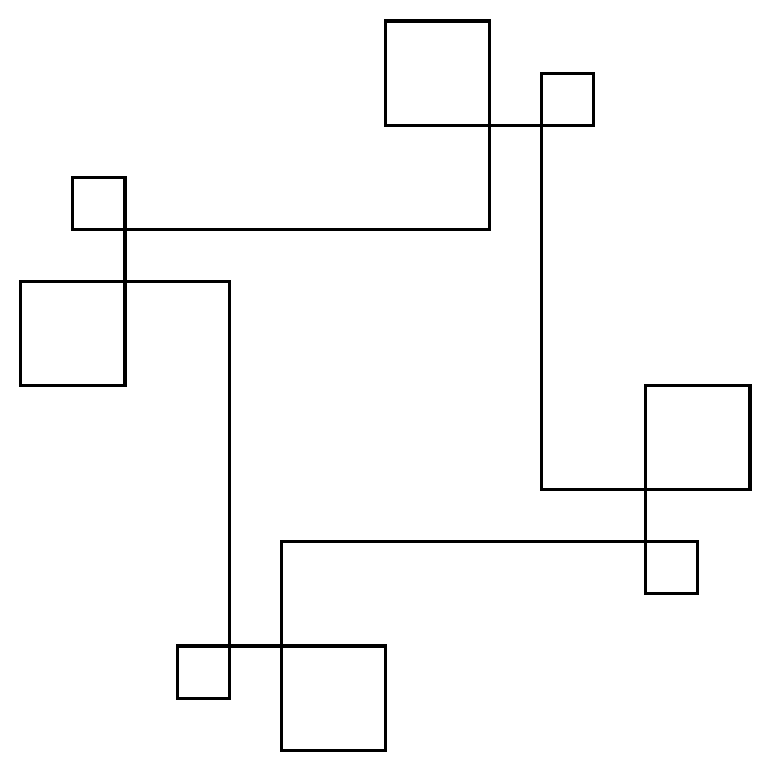
\includegraphics[width=5cm]{artNouveauFourScr}}{An art nouveau picture frame}\label{scr:126}
| pica | 
pica := Bot new. 
4 timesRepeat: [ pica pattern ; go: 50 ]
\end{scriptfigwithsize}

At this point, the astute reader might ask, Why don’t we create a method, named \ct{frame50}, 
for example, corresponding to that of Script~\ref{scr:126}? This is indeed possible, since \emph{any method 
created for a robot can be reused by another robot method}. Creating such methods is the topic 
of the next chapter. 

\begin{exonofigtitle}{A Method for the Art Nouveau Picture Frame}
Create a method named \ct{frame50} that produces the design produced by Script~\ref{scr:126}.
\end{exonofigtitle}

\section{Summary} 

\begin{itemize}
\item A \emph{method} is a named sequence of expressions. It is composed of a name, a comment, 
and a sequence of expressions. Once a method for robots has been defined, any robot 
can execute it in response to a message with the same name. 
\item A method name should always represent what the method does, not how it does it. 
\item A new method for a robot is created using a Class Bot Browser, which is a special editor 
for defining methods. 
\item Inside a method, the variable \ct{self} represents the object that receives the message. 
When the method’s code needs to send a message to the receiver, the message should 
be sent to \ct{self}.
\end{itemize}

\section{Glossary} 


\begin{description}
	\item[Method categories.] A method category is a folder in which methods are sorted. Categories 
help you to find methods more quickly. 
	
	\item[Method.] A method represents a sequence of expressions that an object can execute. 
A method has a name. It is executed when an object receives a message having the 
same name. 

\item[Class Bot Browser.] A Class Bot Browser is a special tool for viewing and editing methods. 

\item[Comment.] A comment is a piece of text surrounded by quotation marks that explains the 
purpose of a method. 

\item[self.] The variable \ct{self} is predefined by Smalltalk. It always represents the receiver of the 
message in a method definition. 
\end{description}

\ifx\wholebook\relax\else
    \end{document}
\fi

%%% Local Variables:
%%% coding: utf-8
%%% mode: latex
%%% TeX-master: t
%%% TeX-PDF-mode: t
%%% ispell-local-dictionary: "english"
%%% End:
